%%%%%%%%%%%%%%%%%%%%%%%%%%%%%%%%%%%%%%%%%
% Large Colored Title Article
% LaTeX Template
% Version 1.1 (25/11/12)
%
% This template has been downloaded from:
% http://www.LaTeXTemplates.com
%
% Original author:
% Frits Wenneker (http://www.howtotex.com)
%
% License:
% CC BY-NC-SA 3.0 (http://creativecommons.org/licenses/by-nc-sa/3.0/)
%
%%%%%%%%%%%%%%%%%%%%%%%%%%%%%%%%%%%%%%%%%

%----------------------------------------------------------------------------------------
%	PACKAGES AND OTHER DOCUMENT CONFIGURATIONS
%----------------------------------------------------------------------------------------

\documentclass[letterpaper]{article}	 % A4 paper and 11pt font size
\usepackage[english]{babel} % English language/hyphenation
\usepackage[protrusion=true,expansion=true]{microtype} % Better typography
\usepackage{amsmath,amsfonts,amsthm} % Math packages
\usepackage[svgnames]{xcolor} % Enabling colors by their 'svgnames'
\usepackage{booktabs} % Horizontal rules in tables
\usepackage[margin=1.0in]{geometry}
\usepackage{xcolor}
\usepackage{float}
\usepackage{alltt}
\usepackage{graphicx}
\usepackage{lastpage} % Used to determine the number of pages in the document (for "Page X of Total")

%----------------------------------------------------------------------------------------
%	TITLE SECTION
%----------------------------------------------------------------------------------------

%----------------------------------------------------------------------------------------

\begin{document}

\begin{center}
    \Large
    \textbf{Assignment 1: \\ Matrix Multiplication}
    
    \vspace{0.4cm}
    \large
        
    \vspace{0.4cm}
    Lara Backer \\ Unmukt Gupta \\ Edward Tremel

\end{center}

%----------------------------------------------------------------------------------------
%  CONTENTS
%----------------------------------------------------------------------------------------

\section{Overview}

Matrix multiplication is one of the most fundamental computations required to solve linear systems, and as such is of vital importance in numerous computational applications. Therefore, reducing computation time for matrix multiplication calculations is an obvious method for increasing the efficiency of many solvers. \\

In this paper, we will be discussing the implementation and results from multiple methods for optimizing matrix multiplication of equation \ref{eq:mm}, with matrix dimensions M, N, and K. Results are compared to often-used matrix multiplication routines, such as those present in BLAS, a basic blocked multiplication method, and a naive matrix multiplication routine. 

\begin{equation}
\text{C (M x N) = A (M x K) * B (K x N)}
\label{eq:mm}
\end{equation}

\section{Optimization Techniques}

\subsection{Blocking}
Blocking techniques take advantage of the temporal locality of inner loops. Each chunk, or 'block', of a matrix, is chosen so that the code loads the necessary block into cache for each loop, discarding the block when the loop is finished. Matrix multiplication is performed block by block. By knowing the cache level sizes, the block sizes can be chosen to fit within the cache and avoid cache misses, which will decrease code performance. \\ 

\noindent Each compute node on the totient cluster used to run this code has an Intel Xeon E5-2620 v3 processor. We first computed the cache sizes to try to figure out the optimal block sizes, as shown in the next subsections. We initially used the results from these calculations for block sizes, but as we will see later, further testing revealed that other block sizes performed even better. 


\subsubsection{Level 1 Cache}
The processor level 1 cache size is 32KB. To fit three blocks for A, B, and C for a square matrix and double matrix values (8 bytes), the formula to compute the optimal desired block size is:

\begin{equation}
\text{3*(block size)$^2$*(double size) = cache size}
\end{equation}

\noindent Thus, the maximum size for this blocking and for square matrices is 36x36.

\subsubsection{Level 2 cache}
For Xeon boards, the processor level 2 cache size is 256KB. In order to optimize for this cache as well, we performed two stages of blocking, one for the level 1 cache (smaller blocks), and one for level 2 (larger blocks). \\ \\

Using the same formula as for the level 1 cache, the maximum size for the level 2 blocking is 103. \\ \\

The first three lines of Figure \ref{fig:progression} show the improvement gained from adding one and two levels of blocking, respectively. We were surprised to see that the second level of blocking appeared to make little difference, but kept it for the small gains it produced at some sizes. 

\begin{figure}[H]
	\centering
	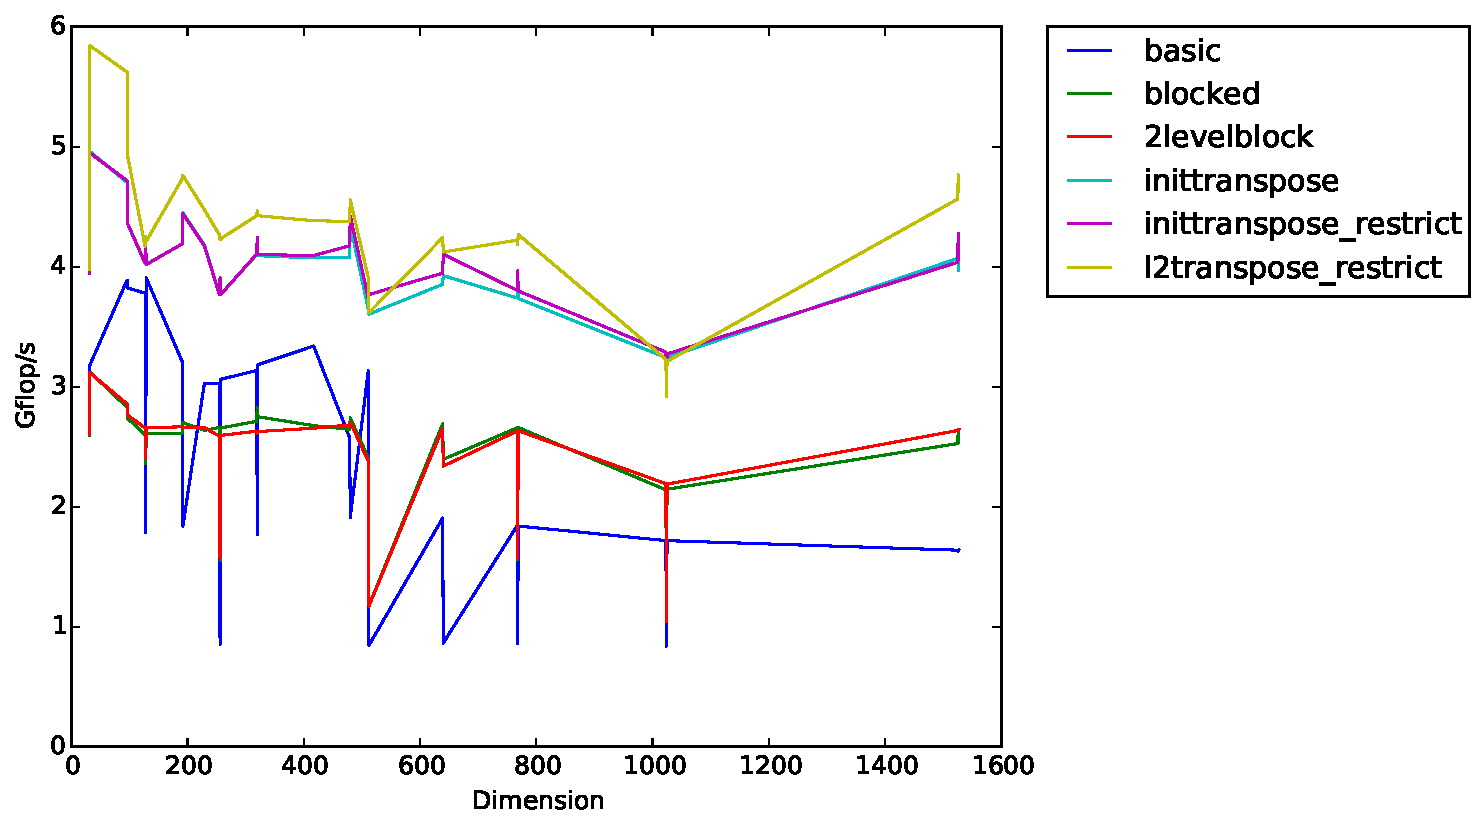
\includegraphics[width=.6\linewidth]{timing-progression.pdf}
	\caption{Performance of a series of optimization techniques. Blocking was performed with 36x36 small blocks and 103x103 large blocks}
	\label{fig:progression}
\end{figure}

\section{Copy Optimization}
Copy optimization improves spatial locality and reduces cache conflicts by copying fixed size blocks and storing them elsewhere for the computation. Due to the additional data storage, it primarily optimizes code for large matrix computations. We used copy optimization on matrix A, since we realized that the pattern of iteration over matrix A would be much more cache-efficient if it was stored in row-major rather than column-major order.

We first tried copying the entire input matrix A into a row-major format before iterating over it in blocks. The results of this optimization are the fourth line on Figure \ref{fig:progression}. As an alternative, to improve spatial locality for the block iterations, we tried copying each large block of matrix A to a row-major format before splitting it into small blocks. This did improve performance compared to transposing the entire input matrix at once, as shown on the last line of Figure \ref{fig:progression}.

\section{Compiler Hints}
C contains some special keywords that can be used to provide hints to the compiler about the layout of memory and allow it to use more aggressive optimizations. We tested the \texttt{restrict} keyword, which specifies that the memory region referenced by a pointer will not overlap with a memory region referenced by any other pointer in scope. This keyword could be applied to all pointers to matrices A, B, and C, since they are allocated in distinct sections of memory and the pointers are never used for any matrix other than their own.

The fifth line on Figure \ref{fig:progression} shows the results of adding the \texttt{restrict} keyword to all applicable pointers in our code that implemented the copy optimization with initial transposing. Unfortunately, this seemed to make little difference, but we kept it in future iterations of the code (such as the copy optimization at the large-block level).

\section{Index Order}
After implementing copy optimization, we tested all index orders for loops in the smallest blocked matrix multiplication routine (\texttt{dgemm\_basic}). We found that the default i,j,k ordering was already optimal for the code and blocking, as it was written.

\section{Block Size Tuning}
Although our calculations showed that block sizes of 36x36 and 103x103 should be optimal for the cache sizes of the cluster's Xeon boards, we experimented with a few other block sizes both smaller and larger than these, after implementing the copy optimization.

The results of different small- and large-block sizes for the implementation that copies matrix A at the large-block level are shown in Figure \ref{fig:l2blocking}. Surprisingly, it appears that the largest two block sizes, 64x64 for the small blocks and 256x256 for the large blocks, resulted in the best performance.

\begin{figure}[H]
\centering
  \centering
  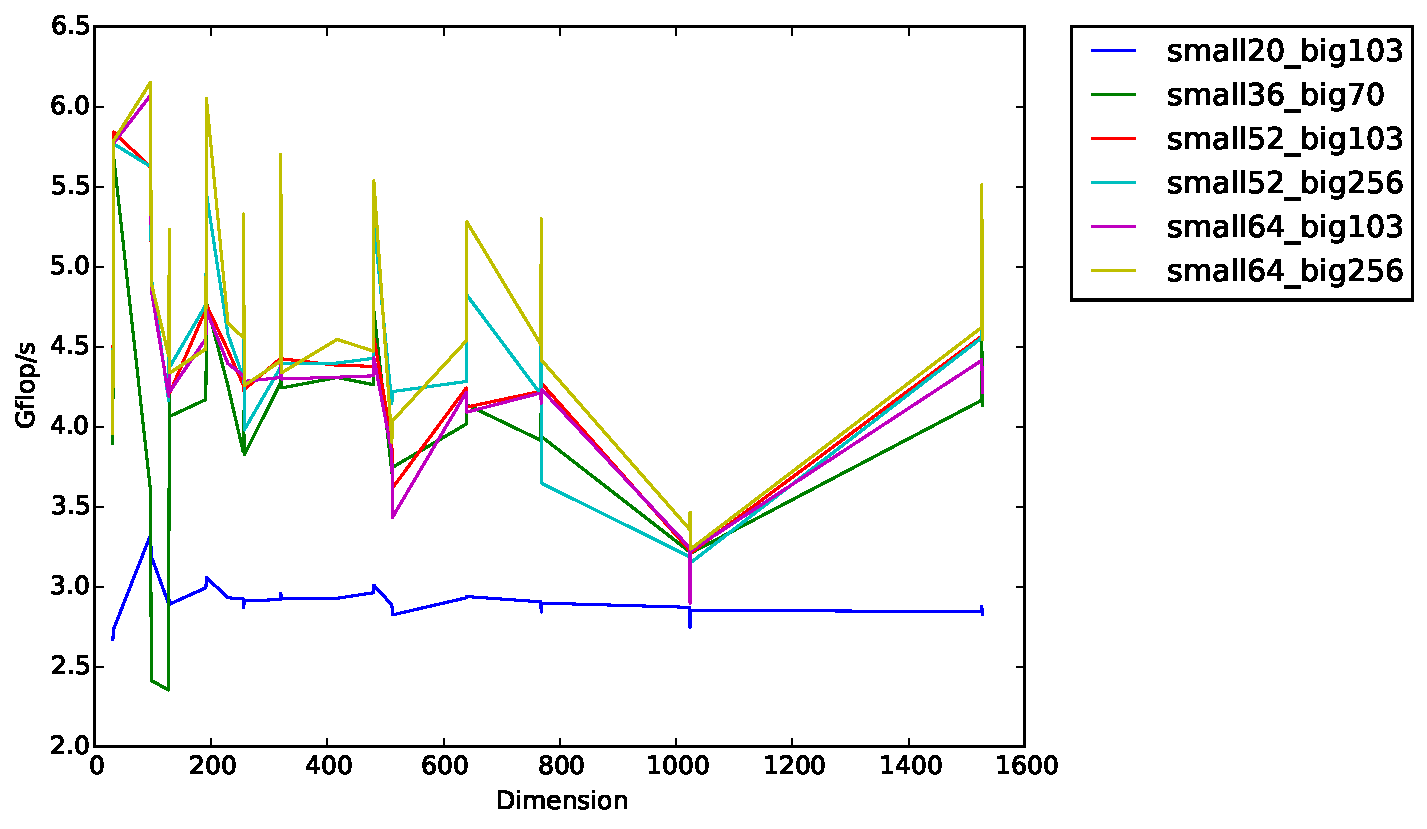
\includegraphics[width=.6\linewidth]{timing-blocksizes-l2transpose.pdf}
  \caption{Comparison of Different Blocking Sizes, with Copy Transpose at Large Blocks}
  \label{fig:l2blocking}
\end{figure}


\section{SSE Directives}

We hoped to be able to use SSE instructions to force matrix C to be written without being cached, since caching C does not improve performance and only takes up cache space that could be used by A and B. We tested a set of Intel intrinsic functions that are documented to use non-temporal storage instructions. We modified \texttt{dgemm\_basic} as follows:

\begin{verbatim}
void basic_dgemm(const int lda, const int M, const int N, const int K,
                 const double* restrict A, const double* restrict B, double* restrict C)
{
    int i, j, k;
        __m128d atemp,btemp,ctemp,cij
    for (i = 0; i < M; ++i) {
        for (j = 0; j < N; ++j) {
            cij = _mm_load_sd(&C[j*lda+i]);
                for(k = 0;k<K;++k) {
                        atemp = _mm_load_sd(&A[k*lda+i]);
                        btemp = _mm_load_sd(&B[j*lda+k]);
                        ctemp = _mm_mul_sd(atemp,btemp);
                        cij = _mm_add_sd(cij,ctemp);
            }
            _mm_stream_pd(&C[j*lda+i],cij);
        }
    }
}
\end{verbatim}

\begin{figure}[H]
  \centering
  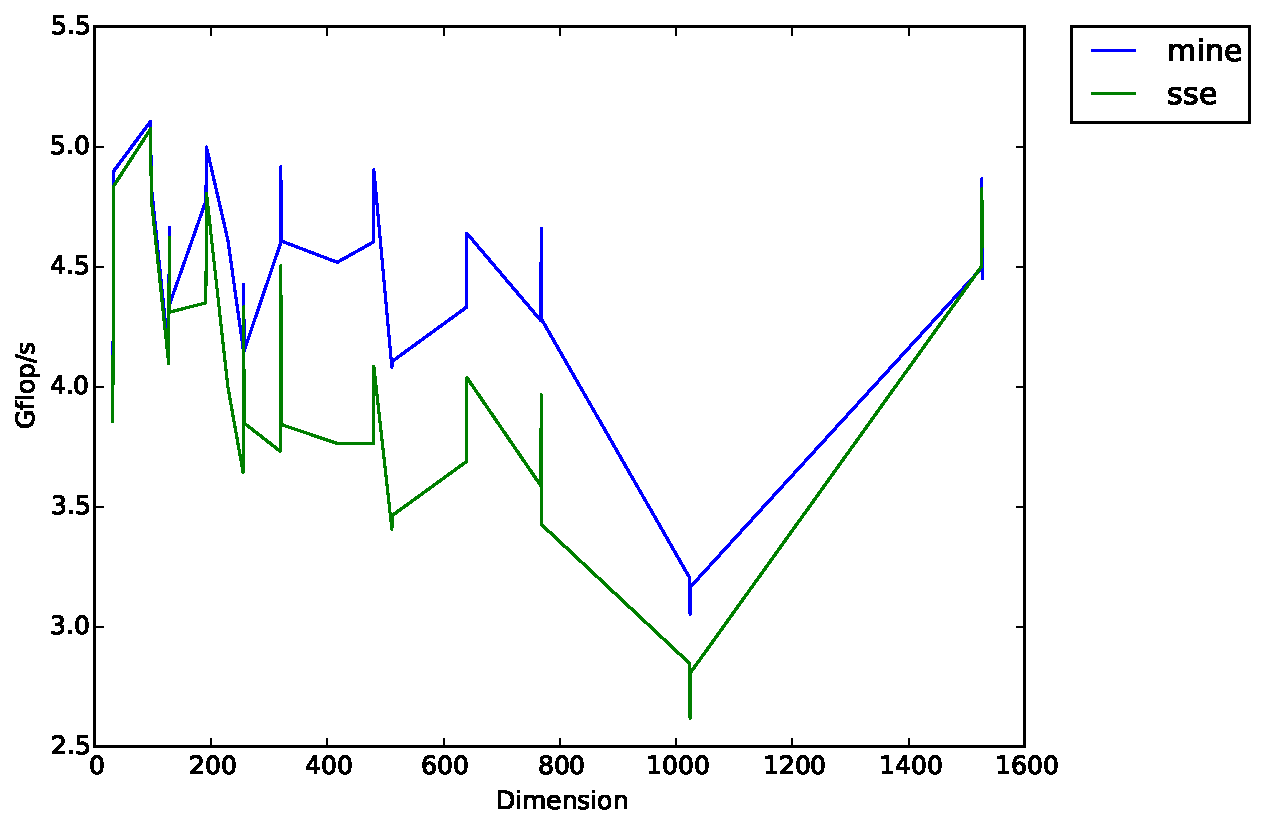
\includegraphics[width=.6\linewidth]{timing_sse.pdf}
  \caption{SSE Comparison Graph}
  \label{fig:sse}
\end{figure}
  
  As can be seen in Figure \ref{fig:sse}, the timings for the modified SSE code were actually worse when compared to the basic blocked dgemm\_mine code. 


\section{Compiler Flags}
Compiler flags that were found to improve performance were for this code are listed as follows: \\
\begin{itemize}
\item -O2: Maximizes speed, enables vectorization. Basic optimize flag. 
\item -mfpmath=sse: Enables XMM registers in floating point operations
\item -Ofast: Enables high level aggressive optimizations -O3, -no-prec-div, and -fp-model fast=2. 
\\ 

Additional options were tested, such as -ipo, -flto, and -march=native. However, none of the flags were actually shown to increase efficiency. A comparison of the timings for options with all bulleted flags (flags), just the -O3 flag (o3), and no flags used (noflags) is shown in Figure \ref{fig:flags}. 

\begin{figure}[H]
\centering
  \centering
  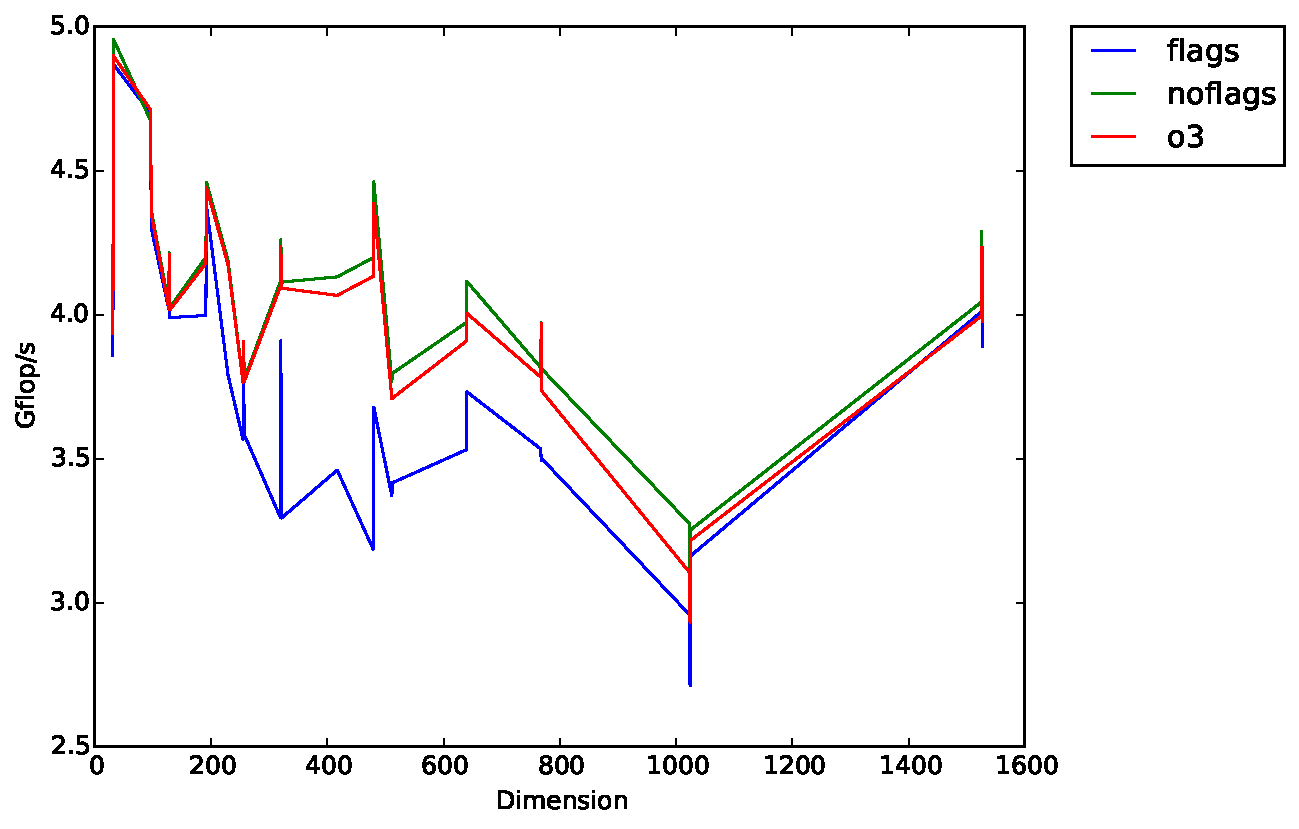
\includegraphics[width=.6\linewidth]{timing_flagcompare.pdf}
  \caption{Flag Comparison Graph}
  \label{fig:flags}
  \end{figure}

\end{itemize}

\section{Conclusion}

After implementing all of the optimizations we found to improve performance, we were able to achieve a performance level a little less than halfway between the naive implementation of matrix multiply and the finely-tuned BLAS library. We also reduced the variation in speed with matrix dimension compared to the naive implementation, smoothing out many of the performance dips at powers of 2. 
The final timing graph for our code is shown in Figure \ref{fig:final}, compared to these two benchmarks.

\begin{figure}[H]
  \centering
  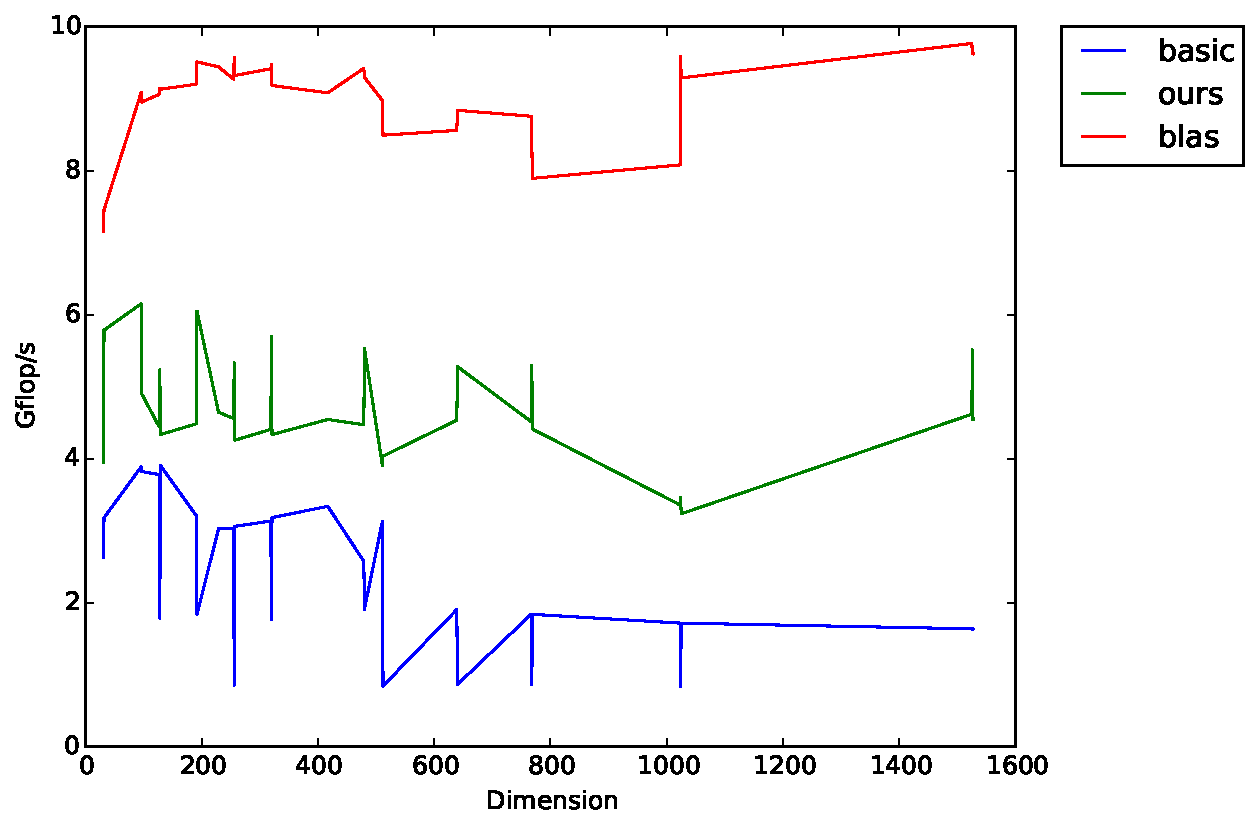
\includegraphics[width=.6\linewidth]{timing-final-comparison.pdf}
  \caption{Our optimized implementation compared to the naive matrix multiply and the BLAS library code.}
  \label{fig:final}
\end{figure}
%----------------------------------------------------------------------------------------

\end{document}
